\section{Empirical Results and Analysis}
\label{cha:results}

%%%%%%%%%%%%%%%%%%%%%%%%%%%%%%%%%%%%%%%%%%%%%%%%%%%%%%%%%%%%%%%
\begin{figure*}[htp!]
\vspace{-1mm}
\hspace{10mm}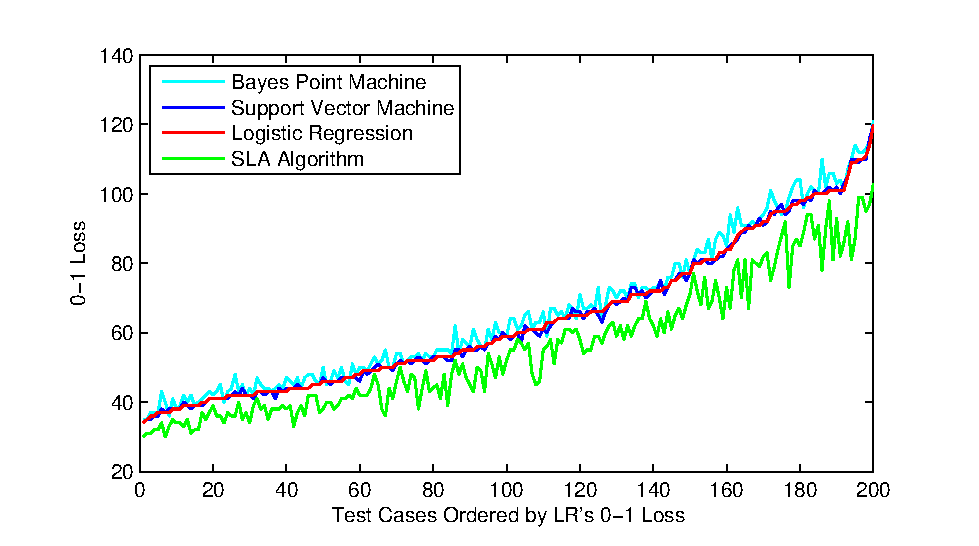
\includegraphics[width=0.45\textwidth]{images/fig61_621a.eps}
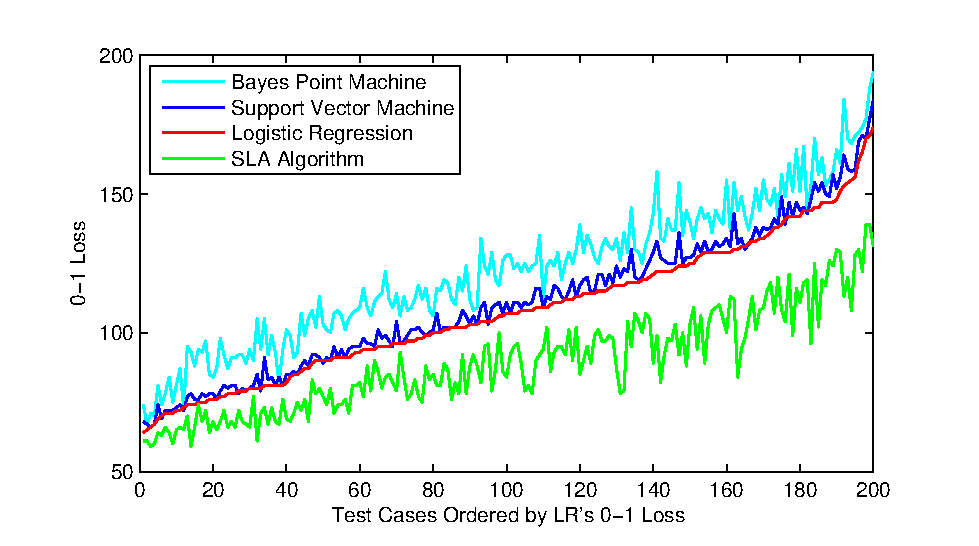
\includegraphics[width=0.45\textwidth]{images/fig61_621b.eps}
\vspace{-2mm}
\caption{ (left) This plot shows the 0--1 loss values by SLA algorithm
  comparing to other methods over 200 synthetic datasets of $N=500,
  D=5$ with optimal 0--1 loss in the range of $[30, 100]$.  
  (right) Same, but in the presence of 15\% noise.}
\label{fig:621a}
\vspace{-2mm}
\end{figure*}
%%%%%%%%%%%%%%%%%%%%%%%%%%%%%%%%%%%%%%%%%%%%%%%%%%%%%%%%%%%%%%%

In this section we evaluate the four previously defined direct 0--1
loss optimization algorithms (BnB, PCS, CSA, and SLA) on a variety of
real and synthetic data.  We compare to SVMs and logistic regression
using LibLinear~\cite{linearSVM}\footnote{
  \url{http://www.csie.ntu.edu.tw/~cjlin/liblinear}}.  We also compare
to the Bayes point machine~\cite{bpm}\footnote{
  \url{http://research.microsoft.com/en-us/um/people/minka/papers/ep/bpm}}
which is a Bayesian approach with connections to the 0--1 loss.

All tests are implemented in MATLAB 7.12.0 running on a 1.7GHz
dual-core i5 Intel processor and 4GB RAM.  Each dataset was normalized
to have all data with zero mean and unit variance in each dimension of
$\x$.  Some tests use real-world datasets taken from the UCI machine
learning repository~\cite{ucidata} and are listed in Table
\ref{tab:losses0noise} along with the relevant number of data $N$ and
dimensionality $D$.

Synthetic testing datasets are generated as follows: (1) A common data
range $R$ is randomly selected between 5 and 10.  (2) Two center points
$C_1, C_2$, each corresponding to one class, are randomly chosen in
the range $\pm (R/2)$ from the origin.  (3) Diagonal covariances in
each dimension of $C_1, C_2$ are specified randomly in range $[1,
  R^2]$.  (4) The desired number of data points for each class are
then generated by a normal distribution with the generated mean
and covariance.

\emph{Noise Generation:} We added noise to some datasets to test
robustness properties of the classifiers.  Noise is generated randomly
and uniformly in the minimum and maximum range $[min -
  0.5(max-min),max + 0.5(max-min)]$ of each dimension of the
dataset and assigned to the first class of the
dataset. Since the range of noise is twice the range of data, this
process produces both background noise and outliers.

%\COMMENT

%\ENDCOMMENT

%%%%%%%%%%%%%%%%%%%%%%%%%%%%%%%%%%%%%%%%%%%%%%%%%%%%%%%%%%%%%%
\begin{table*}[htbp!]
\centering
{\footnotesize 
\begin{tabular}{|c|cc|  ccc|cccc|c|}
\hline\hline
{\bf Dataset} & $N$ & $D$ & {\bf BPM} & {\bf SVM} & {\bf LR} & {\bf SLA} & {\bf CSA} & {\bf PCS} & {\bf BnB} & {\bf Improvement \% }\\ 
\hline 
Breast	& 683 & 10 & 19 & 18 & 19 & 13 		& 13 & 19 & 10 & +44.4\%\\  
Liver	& 345 & 6 & 104 & 99 & 99 & 89 		& 91 & 91 & 95 & +10.1\%\\   
Cmc	& 1473 & 9 & 468 & 464 & 468 & 418 	& 429 & 459 & 459 & +9.9\%\\   
Heart  	& 270 & 13 & 38 & 39 & 39 & 27 		& 31 & 33 & 25 & +34.2\%\\  
Indian  & 583 & 10 & 153 & 154 & 154 & 146 	& 154 & 154 & 148 & +4.6\%\\    
Pima 	& 768 & 8  & 164 & 166 & 166 & 156 	& 157 & 159 & 161 & +4.9\%\\    
Sonar  	& 208 & 60 & 16 & 0 & 0 & 0 			& 0 & 0 & 0 & 0\%\\ 
\hline
\end{tabular}}
\caption{0--1 loss values of comparing algorithms on original
  data. Column `{\bf \%}' shows the improvement in percentage of the
  best of novel algorithms (SLA, CSA, PCS, BnB) over the best of
  existing algorithms (BPM, SVM, LR). As can be seen, novel algorithms
  represent a significant improvement in 0--1 loss optimization.}
\label{tab:losses0noise}
\end{table*}
%%%%%%%%%%%%%%%%%%%%%%%%%%%%%%%%%%%%%%%%%%%%%%%%%%%%%%%%%%%%%%%%

%%%%%%%%%%%%%%%%%%%%%%%%%%%%%%%%%%%%%%%%%%%%%%%%%%%%%%%%%%%%%%%%
\begin{table*}[htbp!]
\centering
\begin{tabular}{|cc|  ccc|cccc|c|}
\hline\hline
{\bf Dataset} && {\bf BPM} & {\bf SVM} & {\bf LR} & {\bf SLA} & {\bf CSA} & {\bf PCS} & {\bf BnB} & {\bf Improvement \% }\\
\hline
Breast 	&& 55 & 52 & 51 & 47 		& 39 & 44 & 45 & 23.5\%\\  
Bupa 	&& 154 & 154 & 152 & 104 	& 111 & 102 & 146 & 32.9\%\\   
Cmc 		&& 584 & 585 & 585 & 554 	& 504 & 551 & 597 & 13.7\%\\   
Heart 	&& 56 & 55 & 54 & 45 		& 49 & 54 & 42 & 22.2\%\\  
Indian 	&& 191 & 191 & 188 & 178 	& 188 & 188 & 182 & 5.32\%\\    
Pima 	&& 241 & 235 & 230 & 194 	& 195 & 213 & 221 & 15.7\%\\    
Sonar 	&& 22 & 18 & 19 & 13 		& 19 & 19 & 2 & 88.9\%\\ 
\hline\hline
\end{tabular}
\caption{0--1 loss values when 10\% noise is added to original data.
Column `{\bf \%}' shows the improvement in percentage of the
  best of novel algorithms (SLA, CSA, PCS, BnB) over the best of
  existing algorithms (BPM, SVM, LR).} 
\label{tab:losses1noise}
\end{table*}
%%%%%%%%%%%%%%%%%%%%%%%%%%%%%%%%%%%%%%%%%%%%%%%%%%%%%%%%%%%%%%%%

%%%%%%%%%%%%%%%%%%%%%%%%%%%%%%%%%%%%%%%%%%%%%%%%%%%%%%%%%%%%%%%%
\begin{table*}[htbp!]
\centering
{\footnotesize 
\begin{tabular}{|c|  ccc|cc c| cc|}
\hline\hline
\multirow{2}*{{\bf Dataset}}&\multicolumn{5}{c}{{\bf T1 -- Total Running Time}}&&\multicolumn{2}{c|}{{\bf T0--ReachSol.}}  \\ 
\cline{2-9}
 & {\bf BPM} & {\bf SVM} & {\bf LR} & {\bf SLA} & {\bf CSA} && {\bf PCS} & {\bf BnB}\\  
\hline
Breast & 0.98 & 0.03 & 0.05 & 1.13 & 161.64 && n/a & 3.59 \\  
Liver & 0.28 & 0.01 & 0.01 & 0.39 & 16.11 && 97.07 & 0.17 \\  
Cmc & 1.35 & 0.06 & 0.05 & 1.02 & 312.78 && 252.06 & 153.4 \\  
Heart & 0.40 & 0.02 & 0.03 & 0.77 & 126.52 && 1.24 & 63.56 \\  
Indian & 0.76 & 0.05 & 0.04 & 1.24 & 166.10 && n/a & 0.8 \\  
Pima & 0.65 & 0.03 & 0.04 & 0.89 & 157.38 && 63.30 & 89.89 \\  
Sonar & 0.37 & 0.54 & 0.13 & 4.32 & 302.58 && n/a & n/a \\
\hline
\end{tabular}}
\caption{This table reports running times corresponding to test results 
  given in Table \ref{tab:losses0noise}. T1 is the total running time
  for BPM, SVM, LR, SLA, CSA (these are fast, so not time limited). T0
  is the time to reach the given solutions for PCS, BnB (their running
  time is unknown as they are terminated after 300 seconds). $T0=n/a$
  means the corresponding algorithm could not find any better solution
  than the initial approximation within the given time limit. Note
  that SVM and LR have small, roughly linear running times. 
  Among novel algorithms, it can be seen
  that SLA is significantly faster. }
\label{tab:runningtimes}
\end{table*}
%%%%%%%%%%%%%%%%%%%%%%%%%%%%%%%%%%%%%%%%%%%%%%%%%%%%%%%%%%%%%%%%


%%%%%%%%%%%%%%%%%%%%%%%%%%%%%%%%%%%%%%%%%%%%%%%%%%%%%%%%%%%%%%%%
\begin{table*}[htbp!]
\centering
{\footnotesize 
\begin{tabular}{|cc|  ccc|c|c|}
\hline\hline
{\bf Dataset} && {\bf BPM} & {\bf SVM} & {\bf LR} & {\bf SLA} & {\bf Improvement \%}\\  
\hline
Breast && $8.95 \pm 2.19$ & $8.42 \pm 2.30$ & $8.09 \pm 2.01$ & $6.87 \pm 1.78$ & +15.1\%\\  
Liver && $43.01 \pm 4.81$ & $42.62 \pm 4.93$ & $45.31 \pm 5.00$ & $40.86 \pm 5.71$ & +4.1\%\\  
Cmc && $35.61 \pm 2.41$ & $35.50 \pm 2.36$ & $36.14 \pm 2.37$ & $36.83 \pm 2.47$ & -3.7\%\\  
Heart && $21.14 \pm 4.72$ & $19.35 \pm 4.45$ & $19.42 \pm 4.52$ & $20.14 \pm 4.31$ & -4.1\%\\  
Indian && $26.63 \pm 3.52$ & $26.67 \pm 3.80$ & $27.13 \pm 3.43$ & $26.36 \pm 3.24$ & +2.7\%\\  
Pima && $28.38 \pm 2.99$ & $28.61 \pm 3.11$ & $28.76 \pm 2.97$ & $25.65 \pm 3.17$ & +9.6\%\\  
Sonar && $28.24 \pm 6.60$ & $28.29 \pm 5.90$ & $28.07 \pm 6.26$ & $27.71 \pm 5.67$ & +1.2\%\\  
\hline
\end{tabular}}
\caption{Prediction error rates (given in \%) of each classifier for
  each UCI dataset (with 10\% noise). The improvement column shows the
  percent improvement of SLA over the best result of other methods ($-$
  indicates SLA was worse). It can be seen that SLA offers lower held-out
  test error rates in five of the seven datasets indicating the robustness
  of 0--1 loss on noisy datasets with outliers and effectiveness of SLA
  in finding good solutions to the 0--1 loss optimization problem.}
\label{tab:ucierrorrates}
\end{table*}
%%%%%%%%%%%%%%%%%%%%%%%%%%%%%%%%%%%%%%%%%%%%%%%%%%%%%%%%%%%%%%%%

\noindent\emph{Optimality of Solutions on Real-World Datasets:} We
evaluated various algorithms on the UCI datasets given in Table
\ref{tab:losses0noise}. This test compares the optimality of the returned
solutions of all algorithms: BnB, PCS, CSA, SLA, SVM, Bayes point
machine (BPM), and logistic regression (LR). 
%In this test, datasets
%are tested with each of the algorithms in two scenarios: without noise
%and with 10\% noise.  
The size of the testing datasets do not allow an
exhaustive search, hence a time threshold of 300 seconds is set for
BnB, PCS.  

%\begin{itemize}
%\item 
Table \ref{tab:losses0noise} shows the 0--1 loss values returned by
comparing algorithms for the original training data.  Here we see that all of the
direct 0--1 loss approximation algorithms the BPM and other solutions
based on convex surrogates of 0--1 loss.
%\item 
Table \ref{tab:losses1noise} shows results similar to
Table \ref{tab:losses0noise} except in the scenario where 
10\% noise is added.  Here we see an even strong performance from the
direct 0--1 loss optimization algorithms indicating their robustness
to noise.
%\item 
Table \ref{tab:runningtimes} shows the running time (T1) of BPM, SVM,
LR, SLA, CSA and the time to reach the given solution (T0) of BnB and
PCS.
%\item 
Since SLA has performed with the best optimization results and runs two
orders of magnitude faster than other direct 0--1 optimizers,
in Table \ref{tab:ucierrorrates} we compare it with the BMP, SVM, and
LR for prediction error on held-out test data for each UCI dataset
augmented with noise.  (Without explicit outlier noise, SLA performed
on par with the BPM, SVM, and LR; not shown due to space restrictions.)  
Here, we see that SLA outperforms
the BPM, SVM, and LR on five of the seven data sets indicating its
ability to find good solutions and the robustness of 0--1 loss in the
presence of outliers.
%\end{itemize}

\noindent\emph{Optimality of Solutions on Synthetic Data: } Since SLA
performed best overall, we perform one further analysis to understand
how consistently it outperforms the baselines.  200 synthetic 
datasets have been generated with size $N=500$,
dimensionality $D=5$, and optimal 0--1 loss in the range from 30 to
100. Figure \ref{fig:621a} (left) shows the results of this test and
(right) with 15\% noise added.  Clearly, noise and outliers
adversely affected other algorithms to a greater extent than SLA.

